\section{Einleitung}
\kopfrechts{Einleitung}%
Die Informationsübertragung in unserem Körper wird vom Nervensystem übernommen.
\index{Nervensystem}%
Dies beinhaltet zum Beispiel das vermitteln von Reizen, welche die Augen oder Ohren aufgenommen haben,
an das Gehirn und das Senden von Befehlen vom Gehirn an die Muskeln.
Das Nervensystem besteht aus Nervenzellen, welche elektrische Signale generieren, von anderen Zellen aufnehmen und weiterleiten können.
\index{Nerbenzelle}%
Die Signale werden so von einer Zelle zur nächsten Zelle weitergeleitet, bis das Signal am Zielpunkt ist.
\subsection{Biologische Grundlagen}
In Abbildung \ref{fig:Aufbau Nervenzelle} ist der Aufbau einer Nervenzelle ersichtlich. 
\begin{figure}
    \centering
    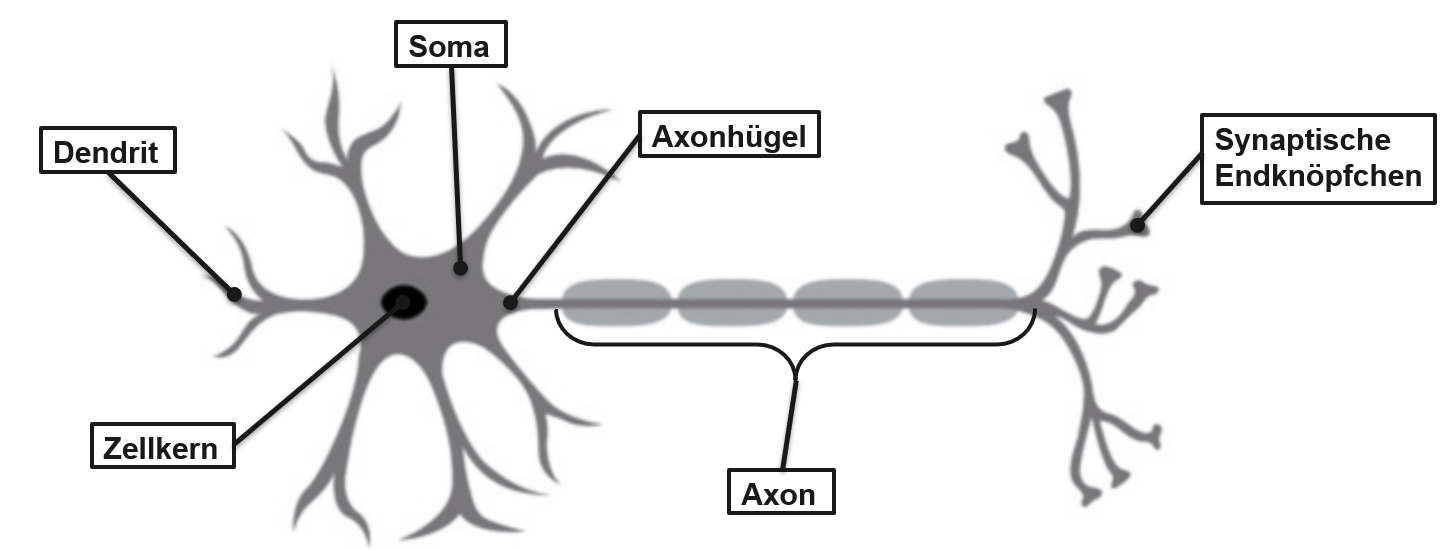
\includegraphics[width=\textwidth]{papers/nerven/Bilder/NervenAufbau2.png}
    \caption{Aufbau einer Nervenzelle nach \cite{nerven:rosadu.}}
    \label{fig:Aufbau Nervenzelle}
\end{figure}


Die Dendriten empfangen Signale. 
\index{Dendrit}%
Im Axonhügel im Soma werden basierend auf den empfangenen Singalen elektrische Impulse erzeugt und mithilfe des Axons übertragen.
\index{Axon}%
\index{Soma}%
\index{Axonhugel@Axonhügel}%
Die Synapsen sind mit der nächsten Zelle verknüpft und so wird das Signal immer weitergeleitet.
\index{Synapse}%

\subsection{Aktionspotential}
Die Nervenzelle besitzt für das Erzeugen von elektrischen Impulsen,
das von den empfangenen Signalen bestimmt wird, ein interessantes Verhalten.
Um zu verhindern, dass im Axonhügel ungewollte elektrische Impulse entstehen, gibt es einen Spannungsschwellenwert,
den das empfangene Signal überschreiten muss.
Bei Signalen mit zu kleiner Spannung, wird dieses Signal sofort stark gedämpft und führt auch zu keinem elektrischen Impuls.
Wenn der Schwellenwert jedoch vom empfangenen Signal überschritten wird, gibt es sofort einen grossen elektrischen Impuls,
\index{Schwellenwert}%
der entlang des Axons weitergeleitet wird. 
Diesen elektrischen Impuls nennt man Aktionspotential.
\index{Aktionspotential}%
\begin{figure}
    \centering
    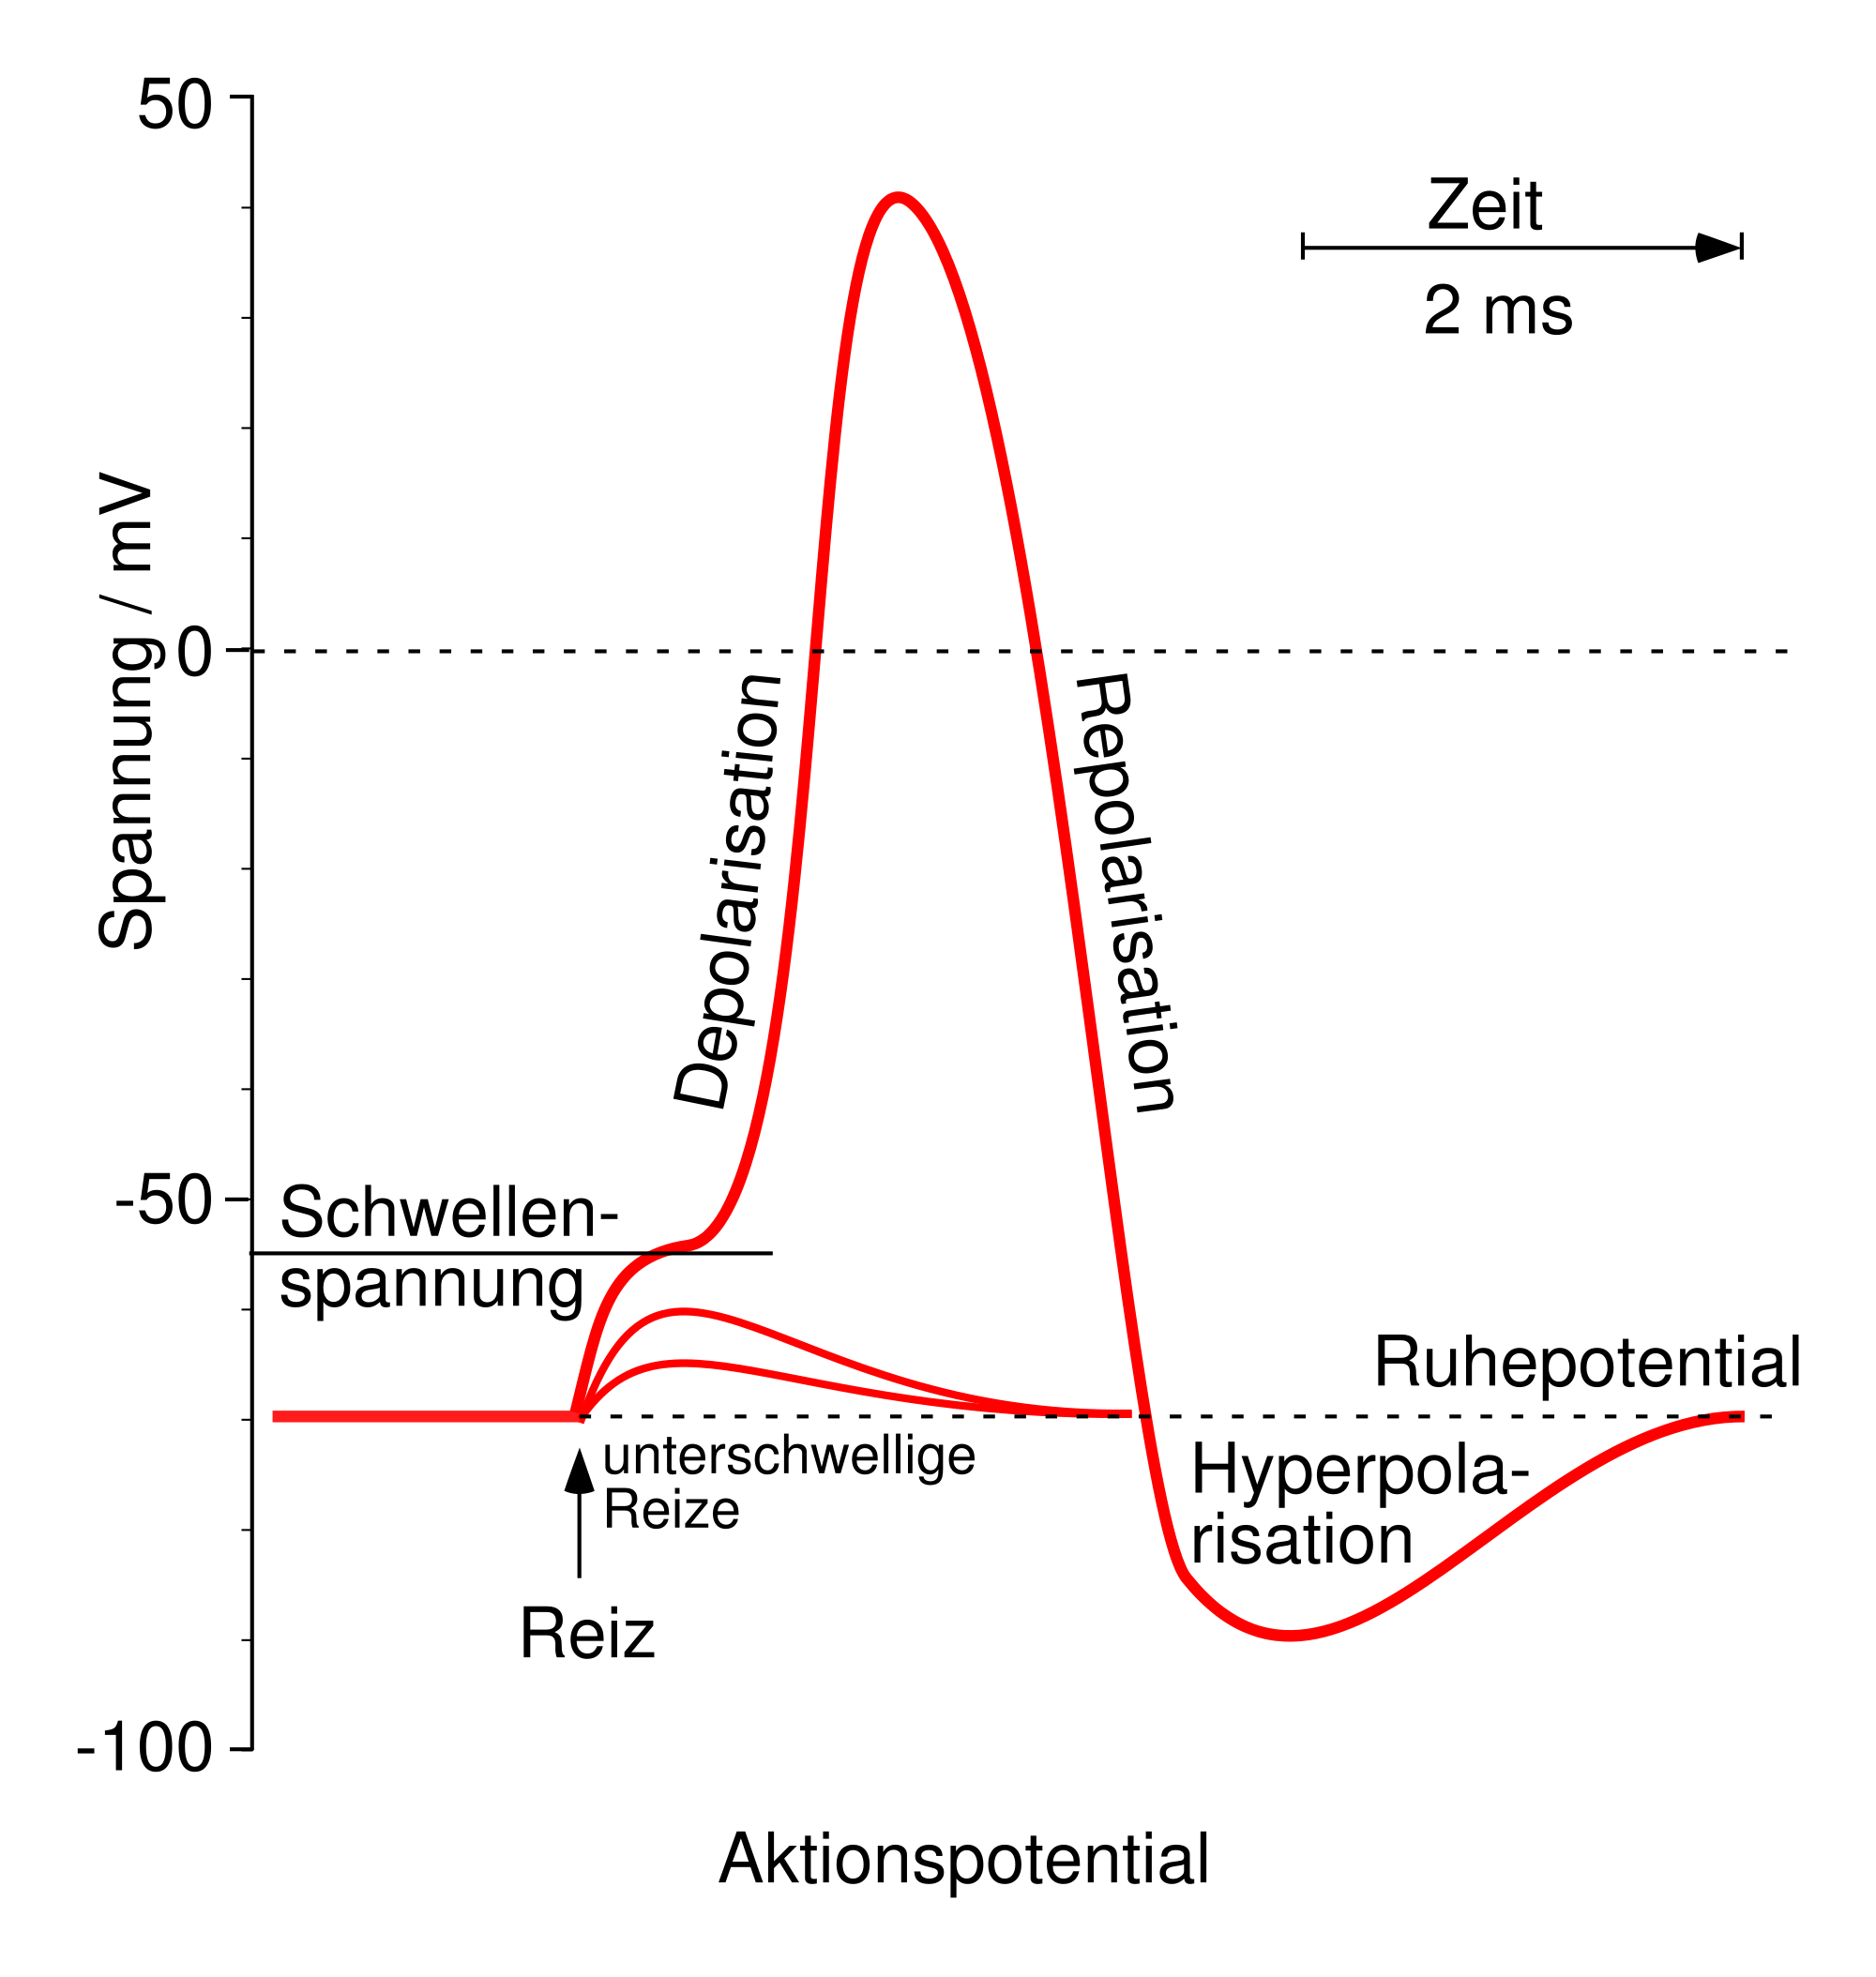
\includegraphics[width=0.7\textwidth]{papers/nerven/Bilder/Aktionspotential.png}
    \caption{Aktionspotential \cite{nerven:JohnEcclesAlanHodgkinAndrewHuxley.}}
    \label{fig:Aktionspotential}
\end{figure}


In Abbildung \ref{fig:Aktionspotential} ist ersichtlich, wie ein Aktionspotential entsteht und schnell wieder abklingt.
Dabei besitzt diese Nervenzelle eine Ruhespannung von $-70$ Millivolt und einen Spannungsschwellenwert von $-50$ Millivolt.
Wenn die Nervenzelle einen Reiz in Form eines elektrischen Signales erhält, wird eine Entscheidung getroffen. 
Ist die Spannung des Reizes kleiner als der Spannungsschwellenwert, wird dies als unterschwelliger Reiz bezeichnet und klingt sofort ab.
Ist die Spannung jedoch grösser, kommt das Aktionspotential in die Depolarisationsphase und steigt bis auf 40 Millivolt.
Sobald das Aktionspotential diese maximale Spannung erreicht, beginnt die Repolarisationsphase.
Dies bedeutet, die Spannung des Aktionspotentials nimmt schnell wieder ab und wird mit $-70$ Millivolt noch kleiner als die Ruhespannung.
In der Hyperpolarisationsphase beruhigt sich das Aktionspotential wieder und nimmt die Ruhespannung von $-50$ Millivolt an.
Dieser Ablauf des Spannungsimpulses geschieht in wenigen Millisekunden 
\cite{nerven:InaLammers.31.08.2015}.

\subsection{Biologische Vorgänge}
\begin{figure}
    \centering
    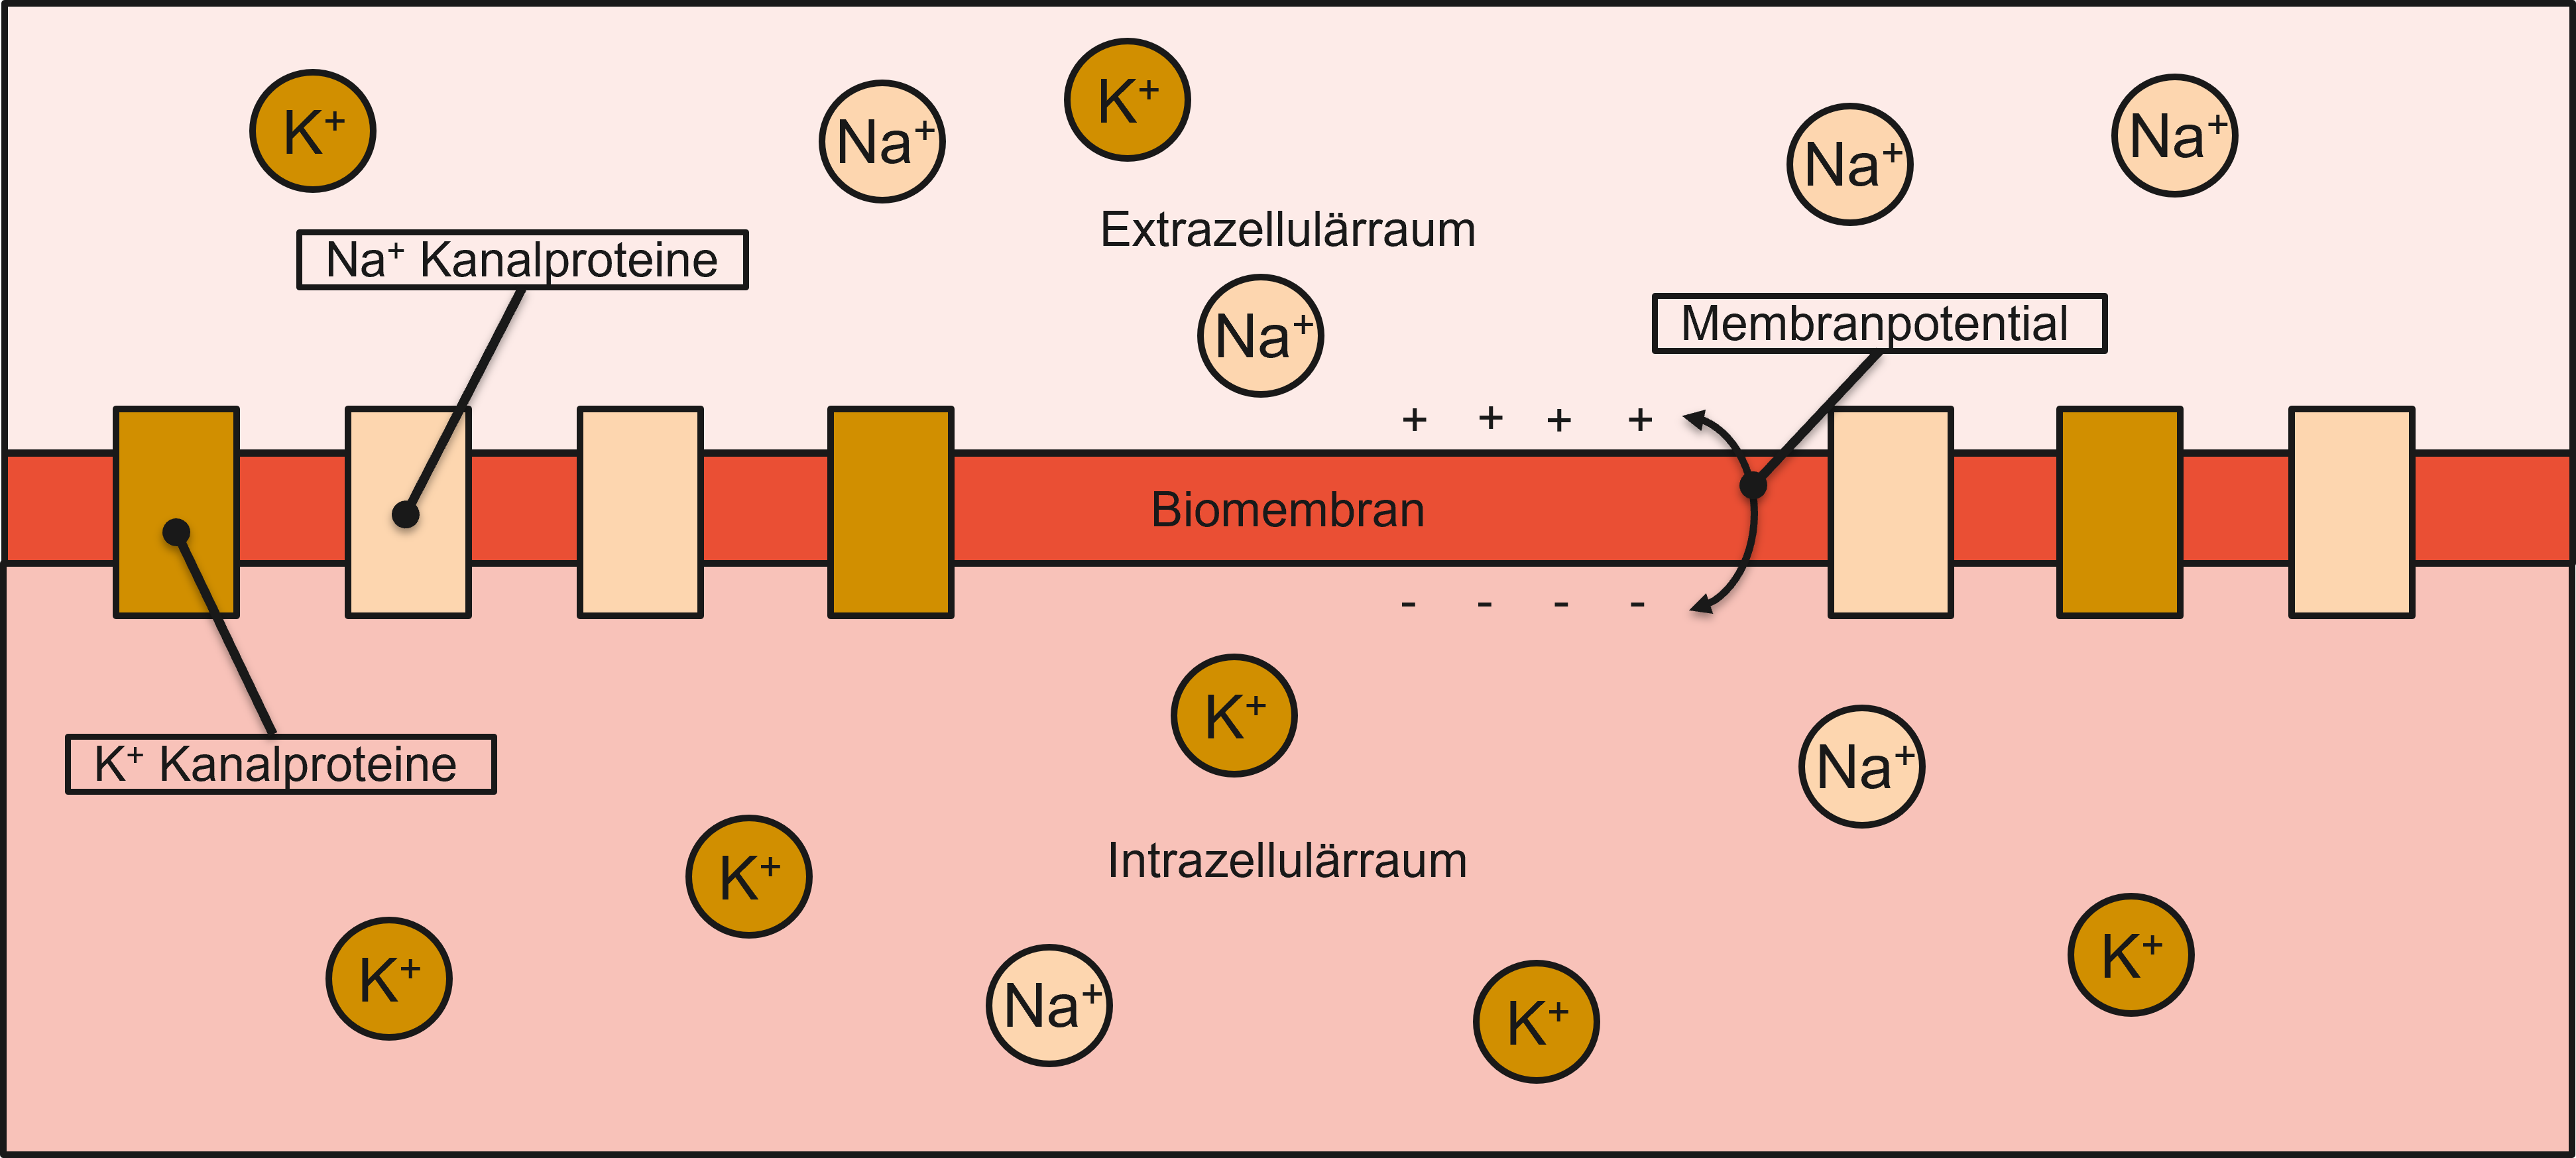
\includegraphics[width=\textwidth]{papers/nerven/Bilder/Vorgang1.png}
    \caption{Ruhezustand: Im Zellinneren tritt eine grössere Kaliumionenkonzentration als im Zelläusseren auf.}
    \label{fig:Ruhezustand}
\end{figure}

\begin{figure}[t]
    \centering
    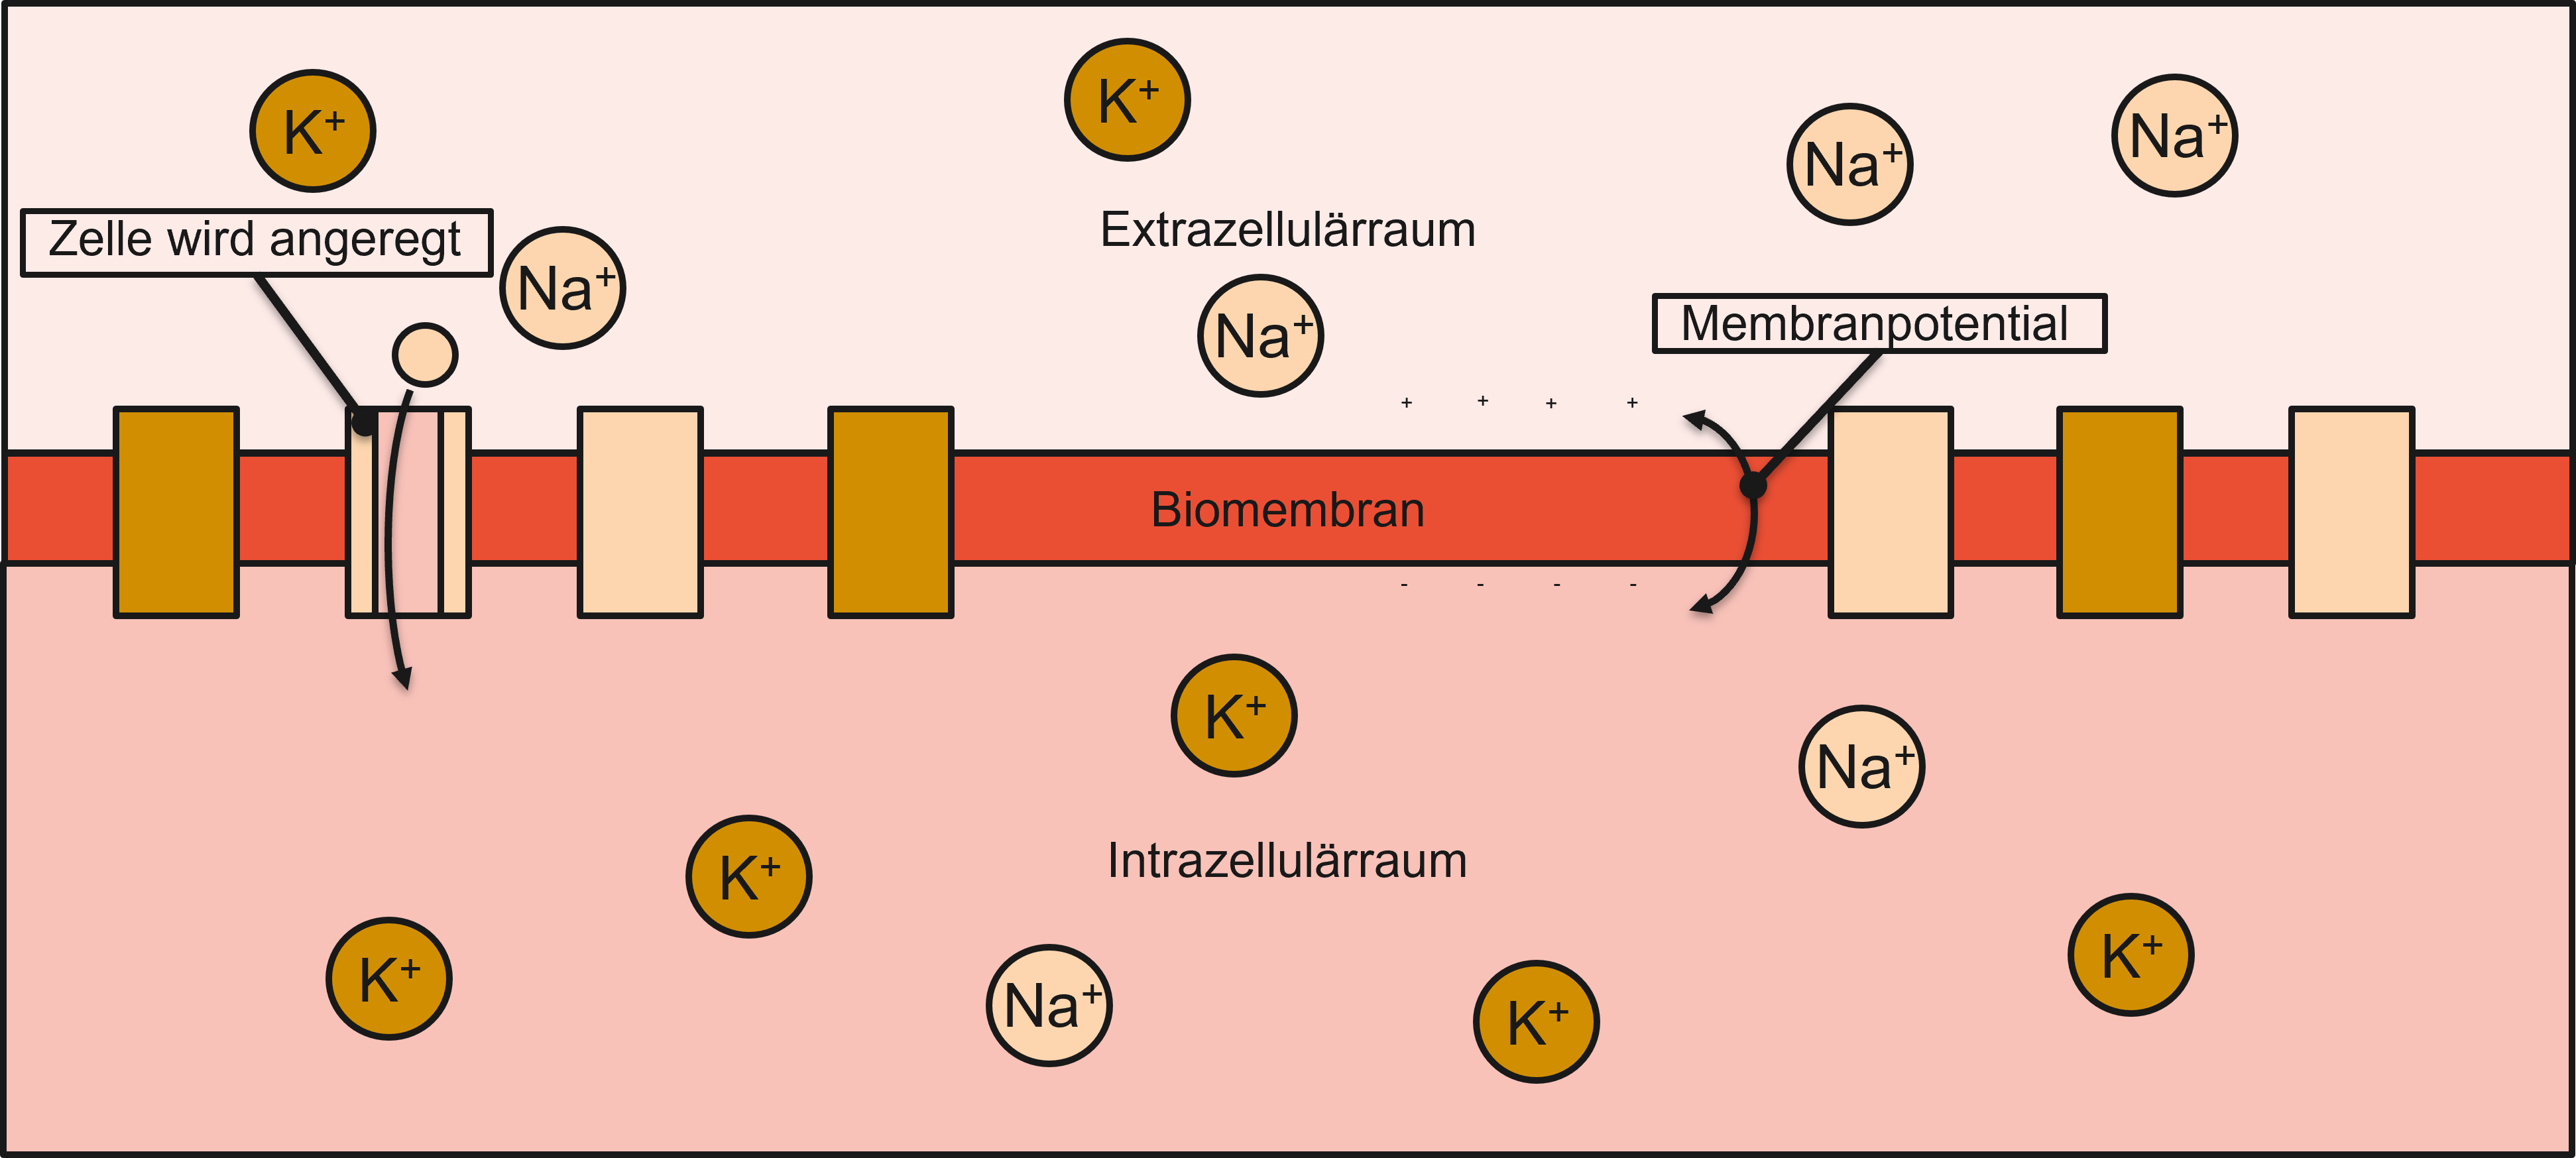
\includegraphics[width=\textwidth]{papers/nerven/Bilder/Vorgang2.png}
    \caption{Anregung: Einige Natriumionenkanalproteine öffnen sich und Natriumionen strömen in die Zelle.}
    \label{fig:Anregung}
\end{figure}

\begin{figure}
    \centering
    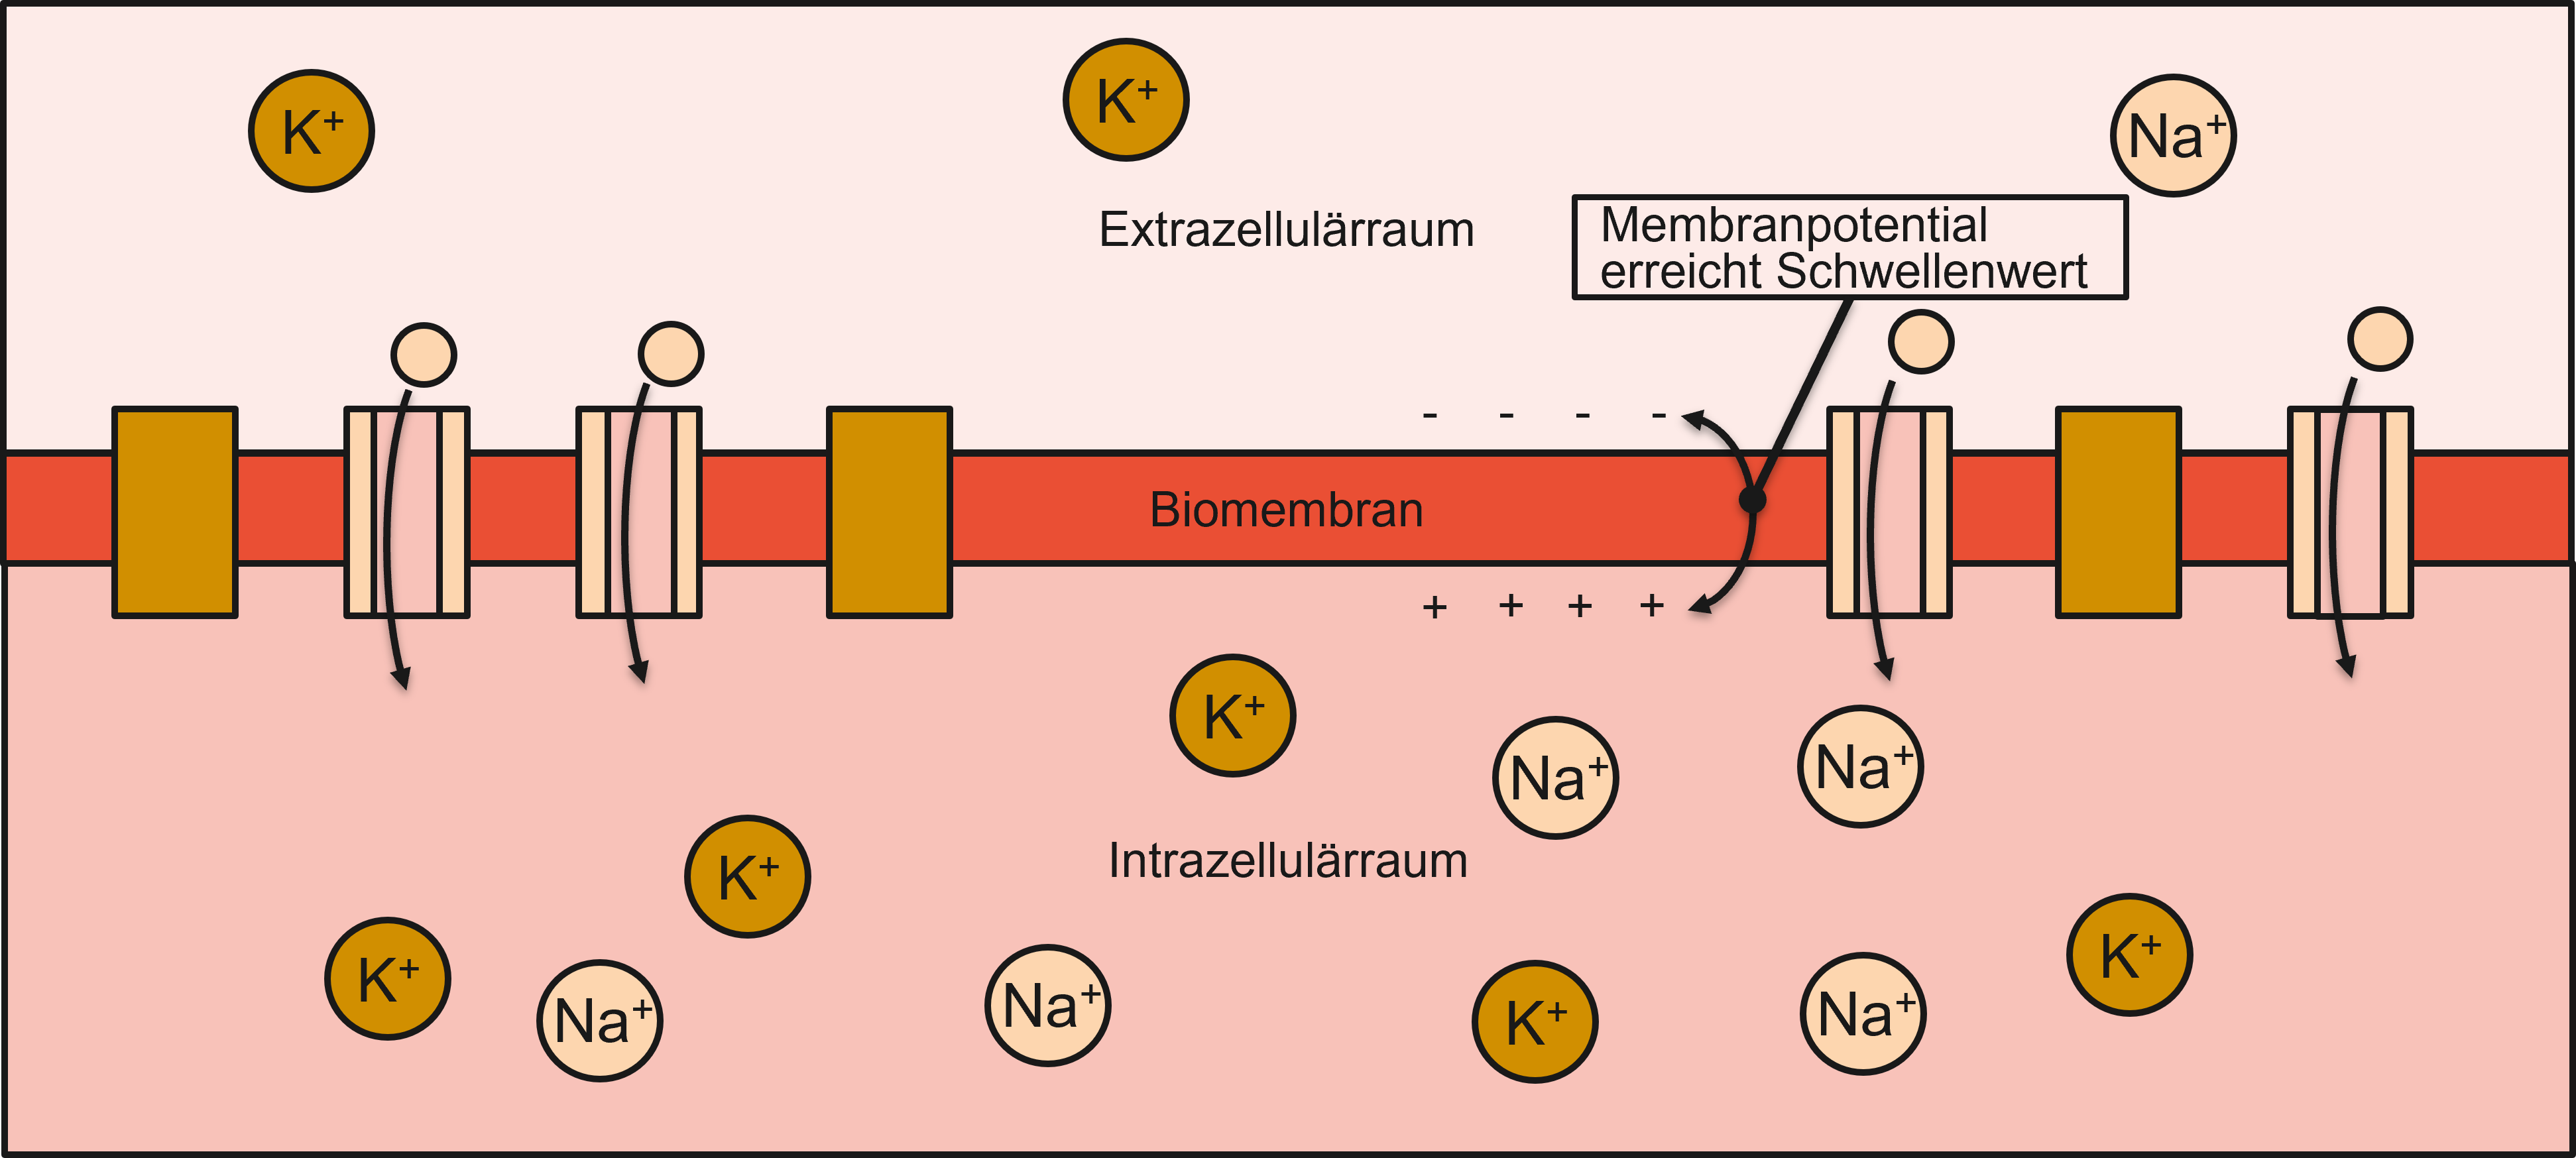
\includegraphics[width=\textwidth]{papers/nerven/Bilder/Vorgang3.png}
    \caption{Depolarisation: Beim Erreichen der Membranschwellenspannung öffnen sich alle Natriumionenkanalproteine und viele Natriumionen strömen in die Zelle.}
    \label{fig:Depolarisation}
\end{figure}

Um dieses Aktionspotential an einer Nervenzelle verstehen zu können, muss die Zellwand betrachtet werden. 
Das Aktionspotential wird durch das Membranpotential beschrieben, dies ist die Ladungsdifferenz zwischen dem Intra- und
Extrazellulärraum.
In Abbildung \ref{fig:Ruhezustand} ist ein Modell der Zellwand einer Nervenzelle im Ruhezustand dargestellt.

Die Ladung von Zellinnerem und Zelläusserem wird durch die Verteilung von positiv geladenen Ionen gesteuert.
Die dafür wichtigsten Ionen sind Kalium- und Natriumionen. 
\index{Kaliumion}%
\index{Natriumion}%
Eine sogenannte Ionenpumpe ermöglicht, dass sich im Ruhezustand der Zelle mehr Kaliumionen im Zellinneren und mehr
\index{Ionenpumpe}%
Natriumionen im Zelläusseren befinden.
Da Kaliumionen eine grössere Ladung als Natriumionen besitzen, ergibt sich so das negative Membranpotential von $-70$
Millivolt.
Die Zellwand besteht aus einer Biomembran, die für Moleküle und Ionen undurchlässig ist.
\index{Zellwand}%
\index{Biomembran}%
In der Zellwand befinden sich jedoch Kanalproteine, die bei der richtigen Anregung spezifische Ionen durch die
\index{Kanalprotein}%
Biomembran transportieren können.

Wenn die Nervenzelle, wie in Abbildung \ref{fig:Anregung}, extern angeregt wird, öffnen sich einige Natriumkanalproteine und transportieren so Natriumionen in
die Nervenzelle.
Durch die Natriumionen vergrössert sich die Ladung der Nervenzelle und das Membranpotential wird somit grösser.
\index{Membranpotential}%

Sobald das Membranpotential grösser als der Schwellenwert von $-50$ Millivolt ist, öffnen sich wie in Abbildung
\ref{fig:Depolarisation} erkennbar schlagartig viele
Natriumkanalproteine und transportieren noch mehr Natriumionen in die Nervenzelle.
Durch diese sogenannte \emph{Depolarisation} erhöht sich die Ladung der Nervenzelle noch stärker und das Membranpotential erreicht ein Maximum. 
\index{Depolarisation}%

Sobald das Membranpotential sein Maximum erreicht schliessen sich die Natriumkanalproteine und dafür öffnen sich die
Kaliumkanalproteine.
Wie in Abbildung \ref{fig:Repolarisation} ersichtlich strömen viele Kaliumionen aus der Nervenzelle hinaus.
In dieser \emph{Repolarisation} nimmt deshalb das Membranpotential schlagartig wieder ab.
\index{Repolaristion}%
\begin{figure}
    \centering
    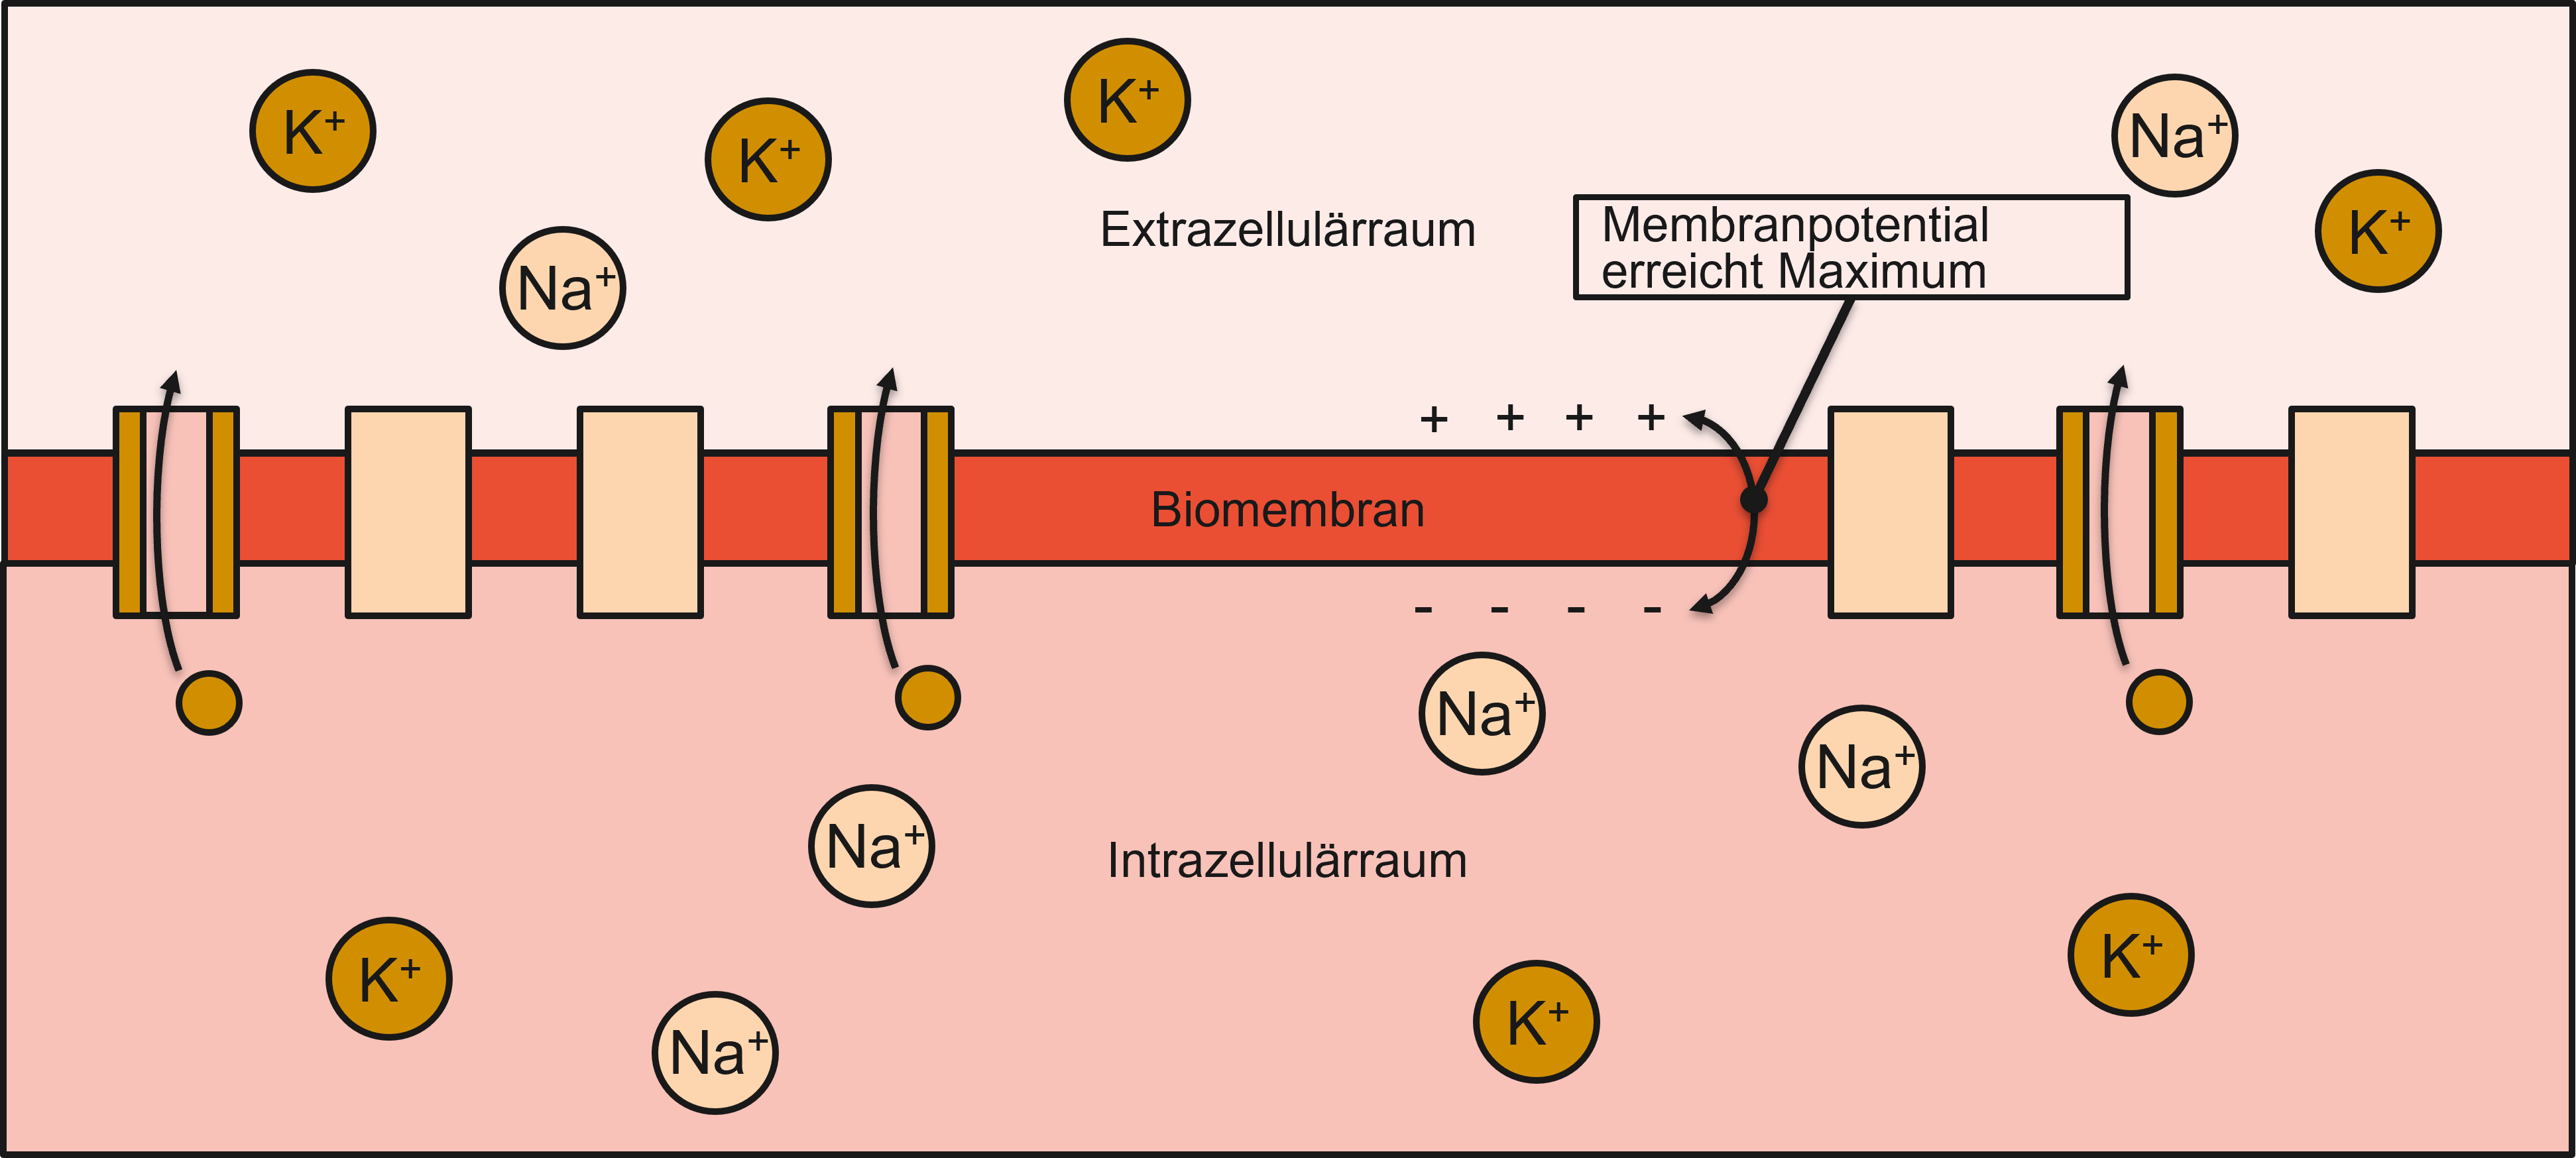
\includegraphics[width=\textwidth]{papers/nerven/Bilder/Vorgang4.png}
    \caption{Repolarisation: Beim Erreichen des Membranspannungsmaximums öffnen sich Kaliumkanalproteine und Natriumionen strömen aus der Zelle.}
    \label{fig:Repolarisation}
\end{figure}


Nachdem das Membranpotential wieder abgenommen hat, muss die Nervenzelle wieder in den Ruhezustand gelangen, dies nennt
man \emph{Hyperpolarisation}.
\index{Hyperpolarisation}%
Dafür öffnen sich, wie in Abbildung \ref{fig:Hyperpolarisation} ersichtlicht, Kanalproteine für beide Ionen und durch die
Ionenpumpe strömen Kaliumionen in die Zelle und Natriumionen aus der Zelle.
Durch die ungleiche Verteilung von Natrium- und Kaliumionen ensteht so wieder ein negatives Membranpotential an der Zellenwand.
\begin{figure}
    \centering
    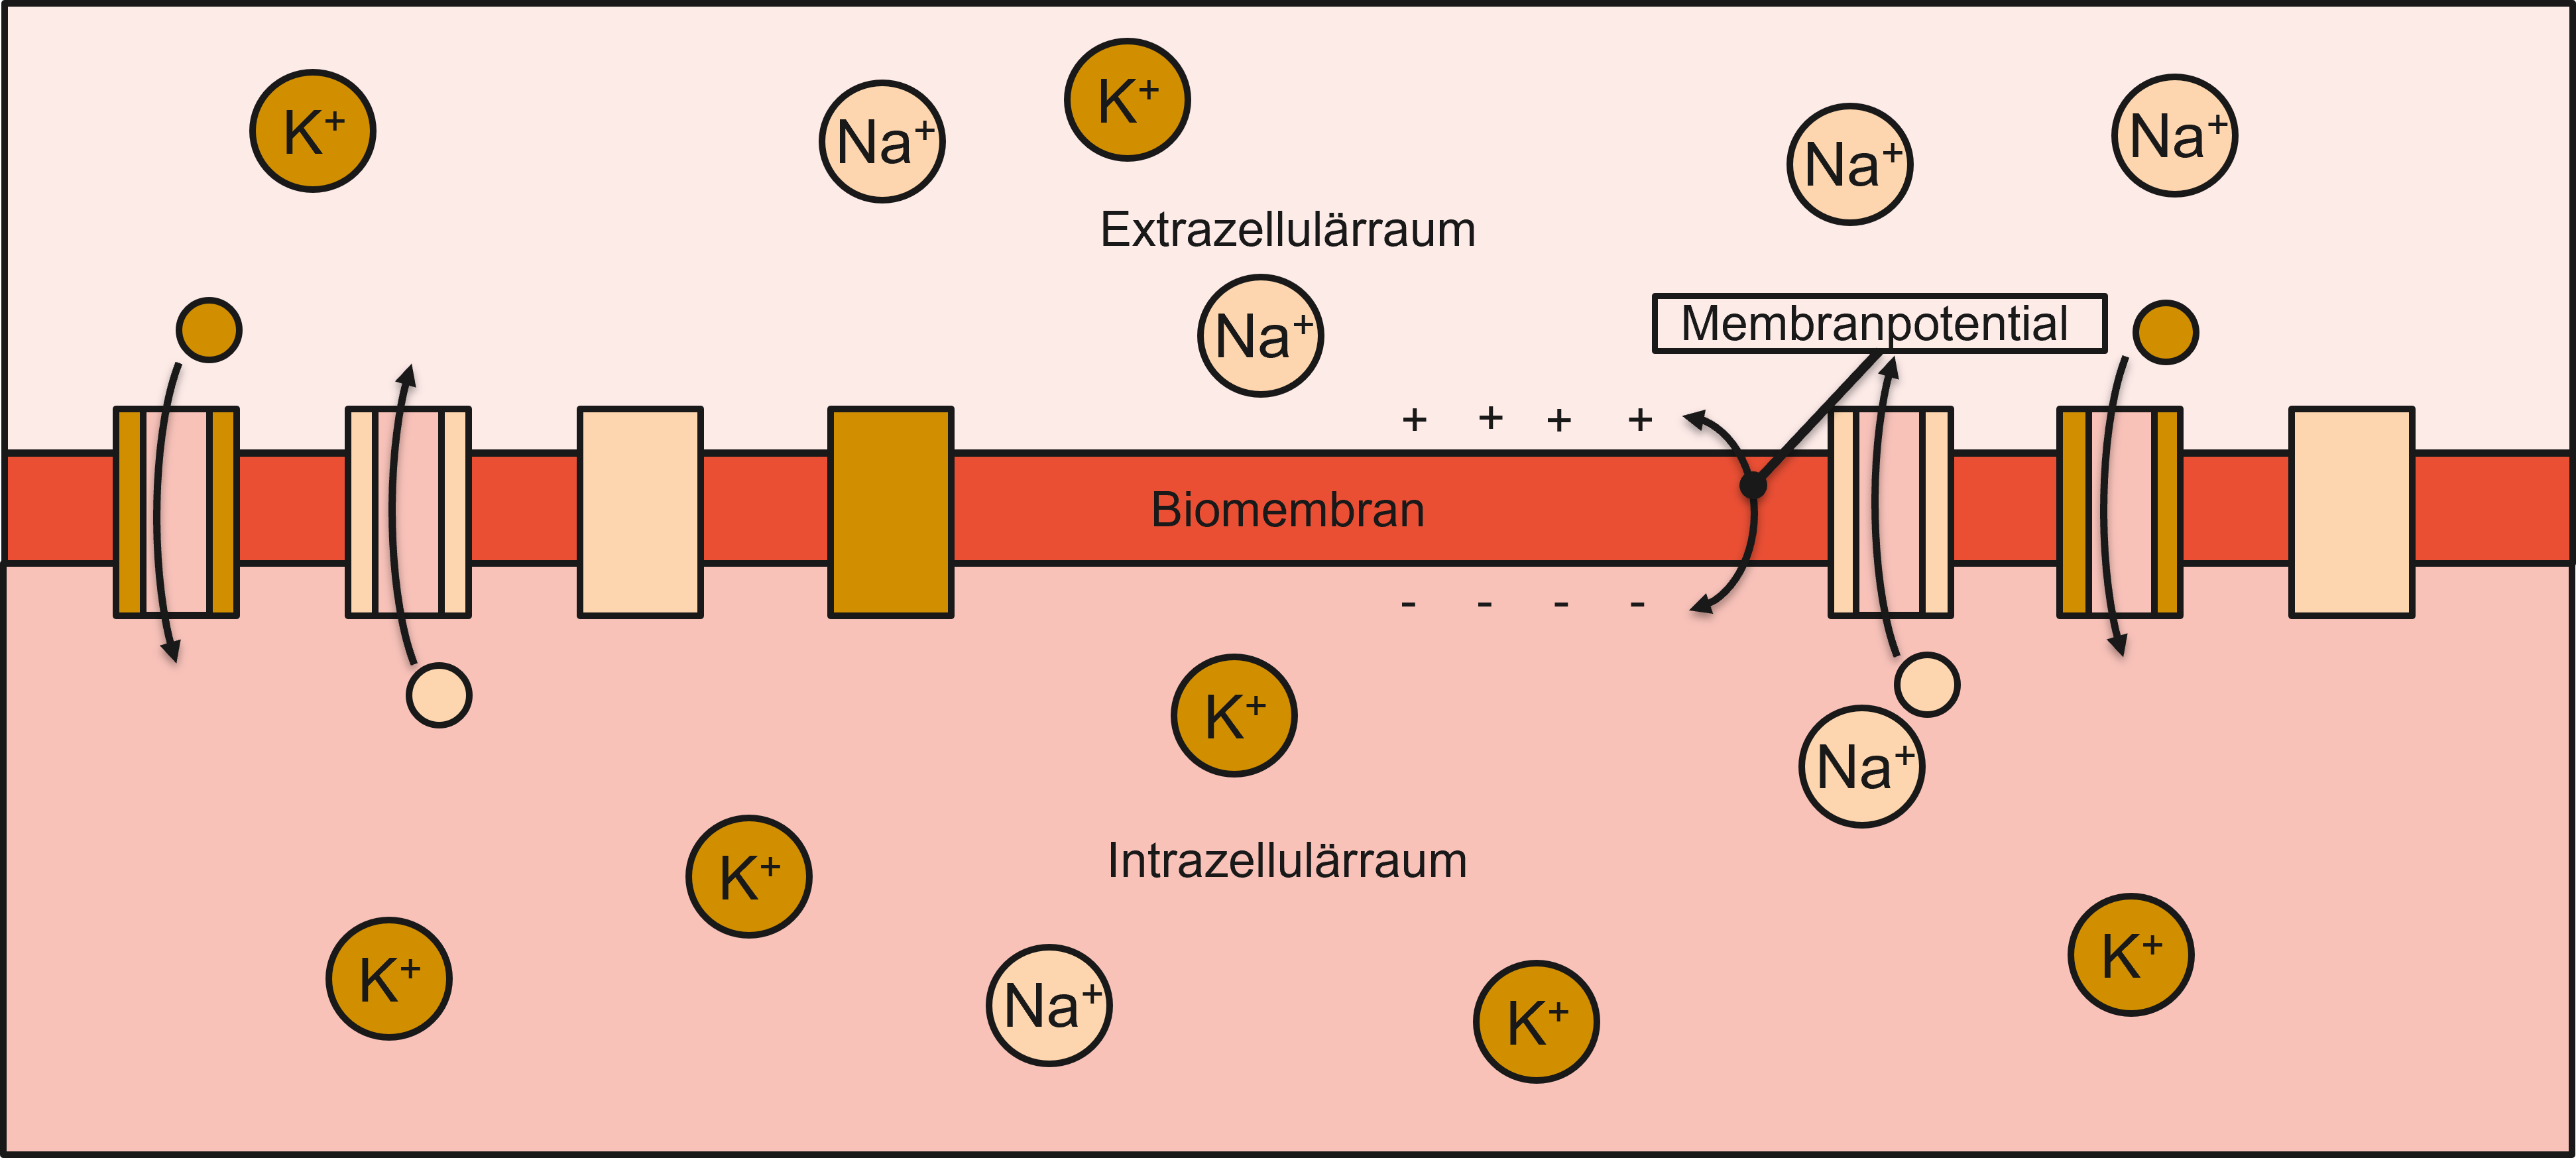
\includegraphics[width=\textwidth]{papers/nerven/Bilder/Vorgang5.png}
    \caption{Hyperpolarisation: Die Nervenzelle gleicht die Ionenkonzentration wieder aus um den Ruhezustand zu erreichen.}
    \label{fig:Hyperpolarisation}
\end{figure}


